\documentclass[a4paper,12pt]{report}
\usepackage[utf8]{inputenc}
%\usepackage[frenchb]{babel}
\usepackage[T1]{fontenc}
\usepackage{lmodern,textcomp}
\usepackage{graphicx}
%\usepackage{listings}
\usepackage{caption}
%\usepackage{fancybox}
\usepackage[pdftex]{hyperref}
%\usepackage{epsfig}
\usepackage{fancyvrb}
\usepackage{tikz}
\usetikzlibrary{shapes.geometric,backgrounds,fit,positioning,trees}
\usetikzlibrary{shapes.callouts}
%\usetikzlibrary{arrows.meta,shapes.callouts}
\usepackage{wrapfig}
\usepackage{manfnt}
\usepackage{dingbat}
\usepackage{xcolor}
\usepackage{geometry}

\definecolor{reddebian}{rgb}{0.84314,0.03922,0.32549}
\definecolor{bluedane}{rgb}{0.09020,0.56863,1}
\definecolor{greendane}{rgb}{0.43137,0.60784,0.14510}
\def\purpledane{violet}

\hypersetup{%
  pdftitle={Xia},
  pdfauthor={Énuma Logiciel Libre},
  pdfsubject={Xia},
  pdfkeywords={Xia, logiciel libre, html5, Inkscape},
  colorlinks= true,
  linkcolor = greendane,
  urlcolor = bluedane
  }

% La dimension des marges
\geometry{hscale=0.7,vscale=0.7}

\title{Xia\\ Create HTML5 "images-actives"}

\renewcommand{\thechapter}{\arabic{chapter}}
\renewcommand{\thesection}{\Roman{section}}
\renewcommand{\thesubsection}{\alph{subsection}}

% pour unifier les indications relatives aux manipulation à effectuer dans les logiciels
% à modifier au besoin
\newcommand{\chemin}[1]{\texttt{\textcolor{reddebian}{#1}}}

% L'environnement alerte                        
\newsavebox{\boiteBrouillon}
\newcommand{\virageDanger}{\textdbend}

\newlength{\LargeurBouleAlerte}
\settowidth{\LargeurBouleAlerte}{%
  
\begin{tikzpicture}%
    \node{\virageDanger};%
  \end{tikzpicture}%
}

% Style pour la boîte alerte
\tikzstyle{boitealerte}=[draw=red,rounded corners,inner xsep=1em,inner ysep=1ex]

% Style pour la boule alerte
\tikzstyle{boulealerte}=[circle,ball color=red,text=white] 

\newenvironment{alerte}{%
  \begin{lrbox}{\boiteBrouillon}% On sauve dans \boiteBrouillon le contenu
    \begin{minipage}{.8\linewidth}%  
      \color{red}%
      \setlength{\parskip}{1ex plus 0.2ex minus 0.2ex}%
}{%
    \end{minipage}%
  \end{lrbox}% Fin. Attention lrbox stocke du contenu sur 1 ligne (pas de paragrpahe)
  % La boîte peut être utilisée via \usebox{\boiteBrouillon}
  \vspace{1.5ex}%
  
\begin{tikzpicture}%
    \node [boitealerte] (cadre) {%
      \hspace{0.5\LargeurBouleAlerte}%
      \usebox{\boiteBrouillon}%
    };%
    \node [boulealerte] (alerte) at (cadre.west) {\virageDanger};%
  \end{tikzpicture}%
  \vspace{1.5ex}%
}        

% L'environnement astuce
\newcommand{\pouceOK}{\large\leftthumbsup}

\newlength{\LargeurBouleAstuce}
\settowidth{\LargeurBouleAstuce}{%
  \begin{tikzpicture}%
    \node{\pouceOK};%
  \end{tikzpicture}%
}

\tikzstyle{bouleastuce}=[circle,ball color=teal,text=white]

\tikzstyle{boiteastuce}=[draw=teal,rounded corners,inner xsep=1em,inner ysep=1ex]
                        
\newenvironment{astuce}{%
  \begin{lrbox}{\boiteBrouillon}% On sauve dans \boiteBrouillon le contenu
    \begin{minipage}{.8\linewidth}%
      \color{teal}%
      \setlength{\parskip}{1ex plus 0.2ex minus 0.2ex}%
}{%
    \end{minipage}%
  \end{lrbox}% Fin. Attention lrbox stocke du contenu sur 1 ligne (pas de paragrpahe)
  % La boîte peut être utilisée via \usebox{\boiteBrouillon}
  \vspace{1.5ex}%
  
\begin{tikzpicture}%
    \node [boiteastuce] (cadre) {%
      \hspace{0.5\LargeurBouleAstuce}%
      \usebox{\boiteBrouillon}%
    };%
    \node [bouleastuce] (astuce) at (cadre.west) {\pouceOK};%
  \end{tikzpicture}%
  \vspace{1.5ex}%
}    

% L'environnement links
\newcommand{\mainDroite}{\large\leftpointright}

\newlength{\LargeurBouleLinks}
\settowidth{\LargeurBouleLinks}{%
  \begin{tikzpicture}%
    \node{\mainDroite};%
  \end{tikzpicture}%
}

\tikzstyle{boulelinks}=[circle,ball color=\purpledane,text=white]

\tikzstyle{boitelinks}=[draw=\purpledane,rounded corners,inner xsep=1em,inner ysep=1ex, align=right]
                        
\newenvironment{links}{%
  \begin{lrbox}{\boiteBrouillon}% On sauve dans \boiteBrouillon le contenu
    \begin{minipage}{.8\linewidth}%
      \color{\purpledane}%
      \setlength{\parskip}{1ex plus 0.2ex minus 0.2ex}%
}{%
    \end{minipage}%
  \end{lrbox}% Fin. Attention lrbox stocke du contenu sur 1 ligne (pas de paragrpahe)
  % La boîte peut être utilisée via \usebox{\boiteBrouillon}
  \vspace{1.5ex}%
  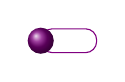
\begin{tikzpicture}%
    \node [boitelinks] (cadre) {%
      \hspace{0.5\LargeurBouleLinks}%
      \usebox{\boiteBrouillon}%
    };%
    \node [boulelinks] (links) at (cadre.west) {\mainDroite};%
  \end{tikzpicture}%
  \vspace{1.5ex}%
}    

\begin{document}
 \maketitle
 \tableofcontents
 
 % il y a, à plusieurs reprises, des paragraphes du style "<à noter"> ou "<astuces">
 % peut-être faut-il adopter le style utilisé pour ce genre de choses dans la doc se3?
 
\section{Introducing Xia}

\subsection{What is Xia ?}

Xia is a free software developed by teachers of french academy of Versailles
It is released under \href{http://www.gnu.org/copyleft/gpl.html}{GPLv3} license.
Xia converter which takes as input a svg file and outputs an image-active in 
html5. Beyond the already known templates export user software ImagesActives 
(\href{http://images-actives.crdp-versailles.fr/spip.php?article11\&lang=fr}
{(accordion, buttons, etc.}), Xia further allows to generate
Interactive activities : games drag and drop, discrimination, selection, etc.

This document will help you "step by step" to create an image-active
Beginning with a simple image-active (crop, comments without particular 
enlightenings), it brings the user to a more complex image-active (multimedia
 enlightenments, games etc.). All examples are on line (each link is written at 
the beginning of the section), and svg source files are also available. At the end
on each part, a heading "Abstract" presents the essential guide lines to 
remember when creating an image-active.

\subsection{General process}

Unlike "ImagesActives", Xia is only needed at the end of the process.
As we can see on illustration \ref{workflowxia}, most of the work is done with 
a  vector graphics editor. We recommend using the free open-source and 
muliplatform software \href{http://www.inkscape.org/}{Inkscape}, which is 
really easy to use (Inkscape will be used in this document).

\begin{figure}[htp]
 \centering
 \caption{Creation process of an image-active with  Xia}
 \tikzstyle{box} = [draw, text width=.6\textwidth, align=center]
 \tikzstyle{ia} = [draw, text width=.8\textwidth, fill=reddebian!80, rounded corners, inner ysep=4mm]
 \tikzstyle{xia} = [draw, text width=.8\textwidth, fill=bluedane!80, rounded corners, inner ysep=4mm]
  % po4a: environement tikzpicture {} 
 \begin{tikzpicture}
   \node[box] (open) {Opening an Image in Inkscape};
   \node[box,below of=open] (create)  {Create details in image};
   \node[box,below of=create] (meta) {For each detail, edit metadata};
   \node[box,below of=meta] (save) {Save project};
   \node[left of=create,xshift=-.37\textwidth, rotate=90] (scape) {\textbf{Inkscape}};
   \begin{scope}[on background layer]
    \node[fit = (open)(meta)(save)(scape), ia] (ink) {};
  \end{scope}
   \node[box,below=2cm of save] (createia) {Create "image-active" in HTML5};
   \node[left of=createia,xshift=-.37\textwidth, rotate=90] (xia) {\textbf{Xia}};
   \begin{scope}[on background layer]
    \node[fit = (createia)(xia), xia] (ink) {};
  \end{scope}
  \draw[-Stealth] (open) -- (create);
  \draw[-Stealth] (create) -- (meta);
  \draw[-Stealth] (meta) -- (save);
  \draw[-Stealth] (save) -- (createia);
 \end{tikzpicture}
 \label{workflowxia}
\end{figure}

\section{Creating your first image-active using Inkscape and Xia: Basic features}

\subsection{Installing Inkscape and Xia}

Having Inkscape and Xia installed on your computer is the only thing you need 
to read this documentation.You will find any relevant information about the 
installation of these softwares on their website :\footnote{See the site 
\href{http://www.inkscape.org/}{Inkscape} and \href
{http://images-actives.crdp-versailles.fr/beta/}{Xia}.}.

\subsection{Building the svg source file to generate an image-active}\label{preparation_svg}

% cette phrase est répétée en début de chaque section: il faudrait trouver un moyen de la mettre en valeur
Explore the \href{http://geoffrey-gekiere.ac-versailles.fr/xia1}{image-active 
created to illustrate this part of the document} and download the \href
{http://geoffrey-gekiere.ac-versailles.fr/xia1/svg/xia1.svg}{svg source file}.

Manipulations described in this section will help you to
create a "basic" image-active featuring:
\begin{itemize}
 \item Zoom-in enabled details
 \item Details comments made only with plain text
\end{itemize}


Once you've chosen the image you will work with, open it with Inkscape 
(\chemin{File} menu, then \chemin{Open}).  When asked by the software
if you wish to "\chemin{Link or incorporate image}", choose "\chemin
{Incorporate}".

Among the many details that one can learn by accessing the 
dialog window \chemin{document} Metadata (\chemin
{File} menu), three will be included in the image-active once
generated : title, creator, rights. Hence it is strongly recommanded
recommended to type in this information. In the following example (see figure \ref{titre_ia}),
we see the importance of a title correctly entered in
Metadata: this is actually the title of the image-active  \footnote{The
fields "author" and "rights" appear in the window
"About", symbolized by a clickable button shaped like the letter "i"}.

\begin{figure}[htp]
 \centering
 \caption{The title entered in the metadata of the document appears above 
the image-active and gives its name to the web page of it. The creator and 
 rights associated appear in the pop up associated with the "i" button 
on the right of the title of the image-active.}
 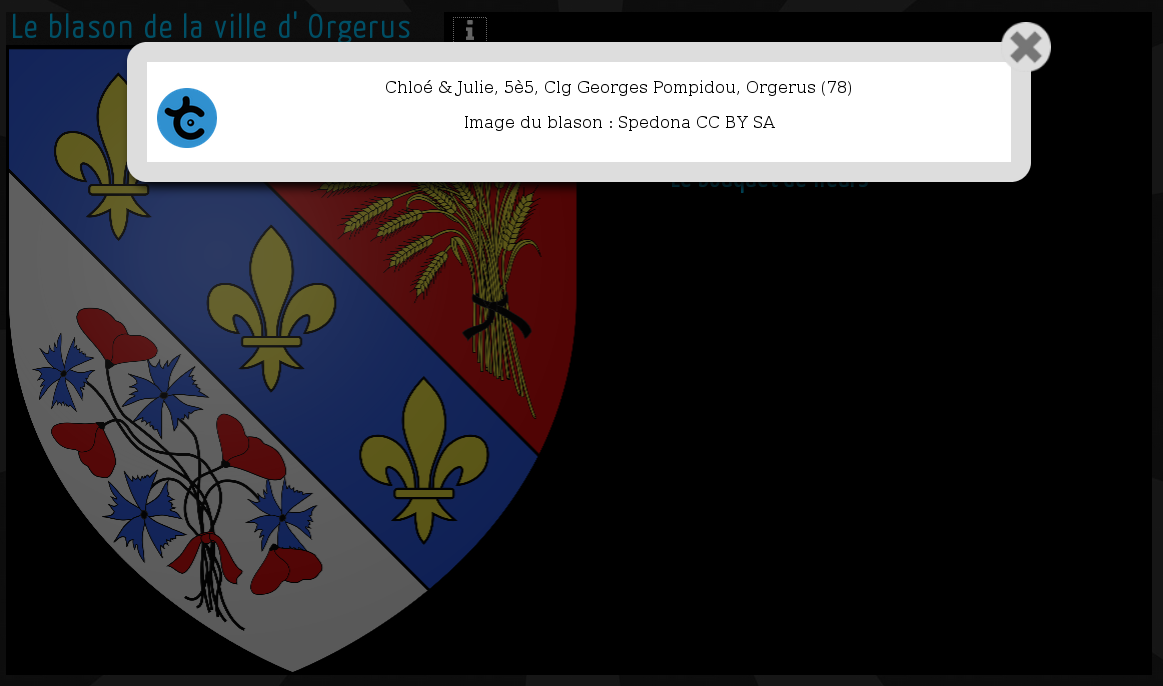
\includegraphics[width=\textwidth]{images/titre_ia}
 \label{titre_ia}
\end{figure}

We can save the image in svg format in the earlywork, 
through the way \chemin{File} menu, then \chemin{Save as\ldots}. 
For more clarity, we will remove the current extension of the image 
in the fields \chemin{Name} of the dialog window. Finally, in the 
dropdown dropdown menu, choose the Inkscape svg file format. \chemin{SVG Inkscape (*.svg)}.

Several Inkscape tools can be used to clip the details that
will become active in the animation generated by Xia . Among these :
\begin{itemize}
 \item 
\includegraphics[scale=0.5]{./images/rec_carre} Tool \chemin{Create rectangles and squares}
 \item 
\includegraphics[scale=0.5]{./images/cercles} Tool \chemin{Create circles, ellipses and arcs}
 \item 
\includegraphics[scale=0.5]{./images/lignes} Tool \chemin{Draw freehand lines}
 \item 
\includegraphics[scale=0.5]{./images/bezier} Tool \chemin{Bezier curves and straight lines}
\end{itemize}

% dans ce paragraphe, peut-être insérer une bidouille quelconque pour que l'allusion aux touches
% Ctrl et Maj soit plus claire (dessiner une touche de clavier?)
Without going in the detail of how these tools work\footnote{For this, 
refer to \href{http://inkscape.org/doc/shapes/tutorial-shapes.fr.html}{Inkscape manual}.}, 
it will be noted that the "\chemin{Create rectangles and squares}" and "\chemin{Create circles, 
ellipses and arcs}"  tools can only be manipulated with the mouse or 
in relation with the keyboard :by pressing the Ctrl key, one draw a square, 
circle or rectangle of dimensions of integer (2: 1, 3: 1, etc.), and 
by pressing the Shift key, draw around the starting point.

The tool "\chemin{Draw Bezier curves and straight lines}" 
allows to crop "click by click" (work points are called 
"nodes").  Figure is closed by clicking on the start node. 
The tool «~Bezier curves~» is called by keeping the mouse button pressed 
after creating a node, then move the cursor to bring up the control handles 
to shape the curve segment as desired.

Note:
\begin{itemize}
 \item if the user sets in Inkscape a left open shape (for
example : a line), Xia will automatically close it  by connecting a 
 straight line between the beginning and the end of it.
 \item The order of creation of details in the image is generated in display 
order of the details (for example, detail first created in
Inkscape appears at the top in the image-active)\footnote{If you wish to 
change that sequence without having to create the details once more, see 
section 
\ref{couche_XML}.}
\end{itemize}

Once a detail is cut out, you can select it with the tool  
\chemin{Select and transform object} to resize it, to" 
move it, etc.

It is with a right click on the cut out detail that you access to 
\chemin{Object properties} (see illustration 
\ref{proprietes_objet}), and 
thus to the dialog window in which you add the text to be associated with the 
detail in the image-active.

\begin{figure}[htp]
 \centering
 \caption{The "Object properties" allows to enter the text that will become a 
 comment for the detail in the image-active}
 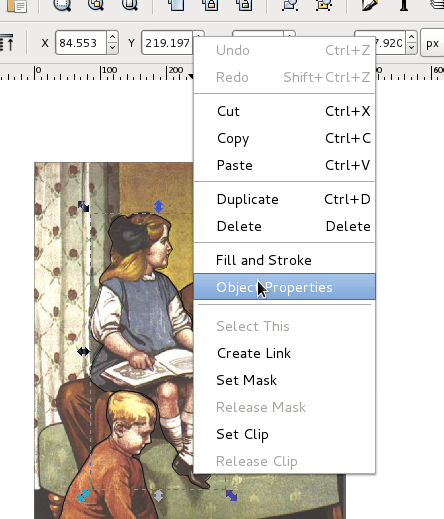
\includegraphics[width=0.5\textwidth]{./images/proprietes_objet}
 \label{proprietes_objet}
\end{figure}

The two fields to be filled in this window are \chemin{Title} and 
\chemin{Description}.  The title filled in here will be the one of the detail, 
description will be its comment.

The process described above must also be done with the background image : 
the title and description indicated here will serve as an introduction to 
the image-active (title and comment not related to a particular detail).

\subsection{Generating the image-active with Xia}

\begin{figure}[htp]
 \centering
 \caption{Xia interface}
 
\includegraphics[width=0.6\textwidth]{./images/xia_vue_generale}
 \label{xia_interface}
\end{figure}

When all the details are clipped and their metadata indicated, one can launch 
Xia (see figure  
\ref{xia_interface}). The first icon on the top left allows 
to select the svg source file.

%\begin{center}
%
\includegraphics[scale=0.4]{./images/xia_open} 
%\end{center}

Clicking on one of the icons export generates a series of files, including a 
\verb|index.html|. 

\begin{alerte}
Warning : this file will not display anything if used 
alone. All the other files and directories generated during the export process 
must be stored in  the same folder as the \verb|index.html| file in order to 
the animation to work properly. \textbf{It is therefore essential to 
dedicate a specific directory for each exported image}. Finally, just open 
the \verb| index.html| file in a web browser to see the image-active.
\end{alerte}

\subsubsection{"Basic" Images actives templates} 
%\begin{tikzpicture}
%  \draw[help lines] (0,0) grid (5,5);
%\end{tikzpicture}

\tikzstyle{box}=[draw, text width=4cm, fill=lightgray!50, rounded corners]
\begin{tikzpicture}
  %\draw[help lines] (0,0) grid (5,5);
  %icons
  \node (bBlue) {
\includegraphics[scale=.3]{./images/buttonBlue}};
  \node[left= .8mm of bBlue, opacity=.5] (aBrown) {
\includegraphics[scale=.3]{./images/audioBrown}};
  \node[right= .8mm of bBlue, opacity=.5] (guClic) {
\includegraphics[scale=.3]{./images/game1clic}};
  \node[below= .2mm of bBlue.south] (pBlue) {
\includegraphics[scale=.3]{./images/popBlue}};
  \node[left= .8mm of pBlue, opacity=.5] (gDDrop) {
\includegraphics[scale=.3]{./images/gameDragAndDrop}};
  \node[right= .8mm of pBlue] (pYellow) {
\includegraphics[scale=.3]{./images/popYellow}};
  \node[above = .2mm of guClic.north] (aCloud) {
\includegraphics[scale=.3]{./images/accordionCloud}};
  \node[above = .2mm of aCloud.north] (aBlack) {
\includegraphics[scale=.3]{./images/accordionBlack}};  
  \node[left = 2cm of aBlack] (files) {
\includegraphics[scale=.3]{./images/xia_open}};
  %comments
  \node[box, text width=2.5cm,above left = 5mm of files] (filesC) {Select the svg source file};
  \node[box,above right = 5mm of aBlack] (aBlackC) {\href{http://geoffrey-gekiere.ac-versailles.fr/xia1/accordionBlack}{accordionBlack}\\ Large comment zone, suitable for insertion of multimedia resources; to be used with vertical images (portrait)};
  \node[box, right = 5mm of aCloud] (aCloudC) {\href{http://geoffrey-gekiere.ac-versailles.fr/xia1/accordionCloud}{accordionCloud}\\ Narrow comment zone, with more space for the image itself ; to be used with horizontal images (landscape)};
  \node[box, below right = 5mm of pYellow] (pYellowC) {\href{http://geoffrey-gekiere.ac-versailles.fr/xia1/popYellow}{popYellow}\\ No lateral comment zone ; 
first click on the detail reveals it, and a second one simultaneously unveils 
the comment and the zoom function zoom on the detail};
  \node[box, left = 25mm of bBlue] (bBlueC) {\href{http://geoffrey-gekiere.ac-versailles.fr/xia1/buttonBlue}{buttonBlue}\\ No lateral comment zone ; 
comments appear above the image (suitable for long comments) ; users access  
comments through icons placed above the image-active};
  \node[box, below left = 5mm of pBlue] (pBlueC) {\href{http://geoffrey-gekiere.ac-versailles.fr/xia1/popBlue}{popBlue}\\ No lateral comment zone; 
first click on the detail reveals it, and a second one pops up the comment 
(no zoom)};
  
  %arrows
  \draw[-Stealth] (aBlackC.south west) -- (aBlack.north east);
  \draw[-Stealth] (aCloudC.west) -- (aCloud.east);
  \draw[-Stealth] (pYellowC.north west) -- (pYellow.south east);
  \draw[-Stealth] (bBlueC.north east) -- (bBlue.north west);
  \draw[-Stealth] (pBlueC.north east) -- (pBlue.south west);
  \draw[-Stealth] (filesC.south east) -- (files.north west);
  
\end{tikzpicture}
% pertinence d'ajouter une 4e colonne pour décrire brièvement les 
% caractéristiques de chaque export?
%\begin{center}
%\begin{tabular}{|c|c|p{3in}|}
%\hline
%Template name & Icon look & What you should know\\

%\hline
%\href{http://geoffrey-gekiere.ac-versailles.fr/xia1/accordionBlack}{accordionBlack}  & \raisebox{-5ex}{
\includegraphics[scale=0.3]{./images/accordionBlack}} & Large comment zone, suitable for insertion of multimedia resources; to be used with vertical images (portrait)\\

%\hline
%\href{http://geoffrey-gekiere.ac-versailles.fr/xia1/accordionCloud}
%{accordionCloud} &  \raisebox{-5ex}{
\includegraphics[scale=0.3]{./images/accordionCloud}}& 
%Narrow comment zone, with more space for the image itself ; to be used with 
%horizontal images (landscape)\\
%\hline

%\href{http://geoffrey-gekiere.ac-versailles.fr/xia1/buttonBlue}{buttonBlue}&  
%\raisebox{-5ex}{
\includegraphics[scale=0.3]{./images/buttonBlue}} & No lateral comment zone ; 
%comments appear above the image (suitable for long comments) ; users access  
%comments through icons placed above the image-active \\
%\hline
%\href{http://geoffrey-gekiere.ac-versailles.fr/xia1/popBlue}{popBlue} & 
%\raisebox{-5ex}{
\includegraphics[scale=0.3]{./images/popBlue}} & No lateral comment zone; 
%first click on the detail reveals it, and a second one pops up the comment 
%(no zoom) \\
%\hline
%\href{http://geoffrey-gekiere.ac-versailles.fr/xia1/popYellow}{popYellow} & 
%\raisebox{-5ex}{
\includegraphics[scale=0.3]{./images/popYellow}} & No lateral comment zone ; 
%first click on the detail reveals it, and a second one simultaneously unveils 
%the comment and the zoom function zoom on the detail\\
%\hline
%\end{tabular}
%\end{center}

\subsection{Abstract}

\begin{enumerate}
 \item An image-active is first build in Inkscape (svg format). Xia only 
 converts the svg source file into an html5 animation
 \item Title of the image-active must be indicated in the \chemin{Metadatas of 
the document}
 \item The text of the details is filled in the \chemin{Object properties}, 
 in the \chemin{Title} and \chemin{Description} fields
 \item General description of the image-active must be indicated in the \chemin
{Object properties} of the background image
\end{enumerate}

\section{Enriched image-active}

Explore the \href{http://geoffrey-gekiere.ac-versailles.fr/xia2}{image-active 
created for this section of the documentation} and download the 
\href{http://geoffrey-gekiere.ac-versailles.fr/xia2/svg/xia2.svg}{svg}.

In this section, the goal is still to create a "traditionnal" image-active 
(ie. in which a detail matches a comment), but the content of the comments 
will be enriched with  formatted text or multimedia resources.

\subsection{Formatting text}

In ordre to insert formatted text, the following tags should be used :

% problème d'alignement du contenu des cellules sur les lignes "<liste de puces"> et "<tracer une ligne">
\begin{center}
 \begin{tabular}{|l|l|}
 \hline
  Tag & Result\\
  \hline
  \hline
  ***bold*** & \textbf{bold}\\
  \hline
  **italic** & \textit{italic}\\
  \hline
  [http://images-actives.crdp-versailles.fr/ Xia website] & \href{http://images-actives.crdp-versailles.fr/}{Xia website}\\
  \hline
  \{\{\{Plain text\}\}\} & \raisebox{-2ex}{
\includegraphics[scale=0.7]{./images/texte_brut}}\\
  % là, faudrait symboliser les espaces simple et double pour les listes de puces
  \hline
  ~* a list\\
  ~* of bullets\\
  ~~* out of 2\\
  ~~* levels\\ & 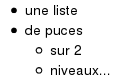
\includegraphics[scale=0.7]{./images/liste_puce}\\
  \hline
  drawing\\
  \verb|----|\\
  a line\\ & 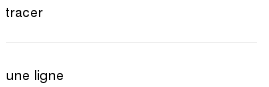
\includegraphics[scale=0.7]{./images/ligne_commentaire}\\
  \hline
  \end{tabular}
\end{center}

\subsection{Inserting multimedia resources into details}\label{enrichissement_multimedia}

Inserting multimedia resources into detail comments is quite easy: just paste 
the resource url (relative or absolute link) or iframe tag of the web service 
you want to use (for example, \href{https://scolawebtv.crdp-versailles.fr/}
{Scolawebtv}).

Xia will automatically create a multimedia player in the comment as long as 
the resource (image, sound or video) matches its supported formats: 
\begin{description}
 \item [Images] jpg, jpeg, png, gif
 \item [Audio] ogg, mp3
 \item [Video] ogv, webm, mp4
\end{description}

The link is just inserted into the thread of comments to the detail:
\begin{description}
 \item[Absolute link] If the resource url is
 
 %\begin{center}
 \verb|http://web.crdp.ac-versailles.fr/02546.ogg|
 %\end{center}
 
 Just type that url inside description of the properties of the object in 
 Inkscape  \item [Relative link] If the multimedia file is located in the image-active 
 folder or in a folder wihtin this one, just indicate its location, keeping in 
 mind that the image-active folder has to be considered as the root folder. 
 For example, if the \verb|video.ogv| file is located in a \verb|videos| 
 folder located itself in the image-active exportation folder, just indicate:
 
 %\begin{center}
  \verb|videos/video.ogv|
 %end{center}
 
  in order to create the player
\end{description}

Since video formats supported by Xia are not natively supported by every web 
browsers, it is recommanded to export videos into the 3 supported formats, 
and to upload them into a single folder (from there, the only difference 
between those files is their extension (ie. .ogv or .mp4 or .webm):\\

\tikzstyle{every node}=[draw=black,thick,anchor=west]
\tikzstyle{auto}=[draw=reddebian,fill=reddebian!30]
\tikzstyle{manual}=[draw=bluedane,fill=bluedane!30]
\begin{tikzpicture}[%
  grow via three points={one child at (0.5,-0.7) and
  two children at (0.5,-0.7) and (0.5,-1.4)},
  edge from parent path={(\tikzparentnode.south) |- (\tikzchildnode.west)}]
  \node [manual] {imageactive\_folder}
    child { node [auto] {index.html}}		
    child { node [auto] {deploy.html}}		
    child { node [auto] {manifest.webapp}}		
    child { node [auto] {css}}
    child { node [auto] {datas}}
    child { node [auto] {font}}
    child { node [auto] {img}}
    child { node [auto] {js}}
    child { node [manual] {videos\_folder}
      child { node [manual] {video.mp4}}
      child { node [manual] {video.ogv}}
      child { node [manual] {video.webm}}
      };
      \end{tikzpicture}

In this example, the files and folders in blue, were manually 
created by the image-active designer and files and folders in red come from the Xia export.
Folder \textcolor{bluedane}
{imageactive\_folder} contains the files et folders generated (in red) by Xia from the 
svg source file, including the \textcolor{reddebian}{index.html} file. The \textcolor{bluedane}
{videos\_folder} was also manually created, in order to host videos inserted 
in the comments of the image-active using relative links.


Thus, even if a particular format is indicated in the description (following 
the previous example : \verb|videos_folder/video.ogv|), if the browser is 
unable to read the resource, it will automatically attempt to read the files 
of the same name possessing a different extension (ie. \verb|video.mp4| 
then \verb|video.webm|).

The last option is to insert in the commentary the iframe code hosting service 
resources. This will be interpreted and the reader will appear in the comment, 
giving access to the resource.

\subsection{The "audioBrown" template: sounds instead of text}

The "audioBrown" template is specifically dedicated to creation of 
images-actives in which details are associated with sounds rather than text.

The method to insert sounds using absolute or relative links is described in 
section 
\ref{enrichissement_multimedia}. If you wish the sound to play 
automatically as the user click on the comment, just add \verb|autostart| right 
after the url \footnote{The "autostart" tag also works with the other 
Xia templates.}:\\"
\begin{center}
 \verb|sons/son_detail_1.ogg autostart|
\end{center}


\subsection{Inserting images into your image-active}\label{insertion_images}

Png images can be added to the background image-active. To do this, in 
Inkscape, go in the \chemin{File} menu, and choose \chemin{Import} 
to incorporate your new image.

Imported image will only appear in image-active if applied white background in 
Inkscape (choose white in the horizontal colour palette at the bottom of 
Inkscape interface (see illustration 
\ref{remplissage_blanc}).

\begin{figure}[htp]
 \centering
 \caption{In Inkscape, select the embedded png then apply a white background 
 by selecting the color from the horizontal colour palette to make it 
 automatically visible} 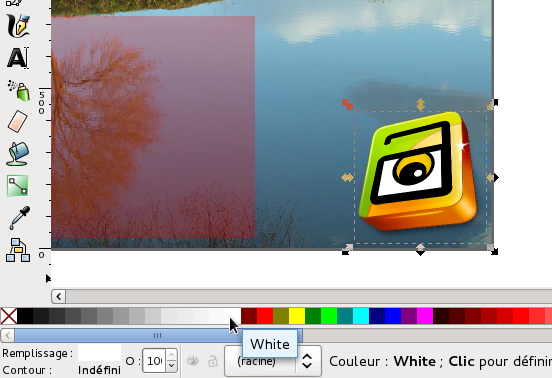
\includegraphics[width=0.6\textwidth]
 {images/remplissage_blanc}
 \label{remplissage_blanc}
\end{figure}

By indicating a URL in the \chemin{Title} of \chemin{Object properties} field, 
the embedded image becomes a clickable icon linking to a web page.

\subsection{Displaying a question and unveiling an answer}

Designer can create an "\textit{Answer}" clickable icon, momentarily 
preventing user to read the end of the comment.

To do so, just indicate, in the description, the line\\ \verb|Answer:| or 
\verb|answer:| followed by the text you wish to be shown.

\subsection{Controlling details behavior : automatic display and disabled zoom}
\label{couche_XML}

Default behavior of details in an image-active consists in:
\begin{itemize}
 \item highlighting details only on mouse over or with a click on the comment 
 detail title
 \item zoom in effect when clicking again on the active detail\footnote{Except 
 for the popBlue template.}
\end{itemize}

Both of these default behaviors can be modified if the designer applies a white
 or black background to cropped details (see section 
\ref{insertion_images} 
 and illustration 
\ref{remplissage_blanc}):
\begin{description}
 \item [Detail with a white background] In the generated image, details will be
 immediately visible in the form of a flat area of opaque color (logically hiding the background image) that once selected, reveals the background image (detail remains zoom-able)
 \item [Detail with a black background] Users still have to click on the detail to unveil it, but it is not zoom-able.
\end{description}

Logical consequence : the designer can not apply a white and a black
background all together on the same detail. The image-active can not be 
both immediately displayed \textit{and} have the zoom effect disabled.

\subsection{Controlling order of details display in the lateral comment zone}

By default, in the image-active, the details appear vertically in the order in which the relevant details have been created (the first detail created in Inkscape corresponding to detail placed up in the sidebar of the image-active).

We will go through the \chemin{XML Editor} in the \chemin{Edit} menu in order to change this default order.

A priori complex to manage, this dialogue window is in fact quite easy to use : selecting the image detail highlights corresponding XML inputs and the only thing left is to drag the files to the desired location (see figure \ref{ordre_couches}).

Thus, the user who frequently changes the order of details should be used to inquire for each the field \chemin{ID} of its properties in in order to be able to more easily handle them in the \chemin{XML Editor}.


\begin{figure}[htp]
 \centering
 \caption{The Inkscape XML editor allows to control the display order of the details in the image-active. Note the highlighting of an element  
in the editor and on the background image by a single mouse click.}
 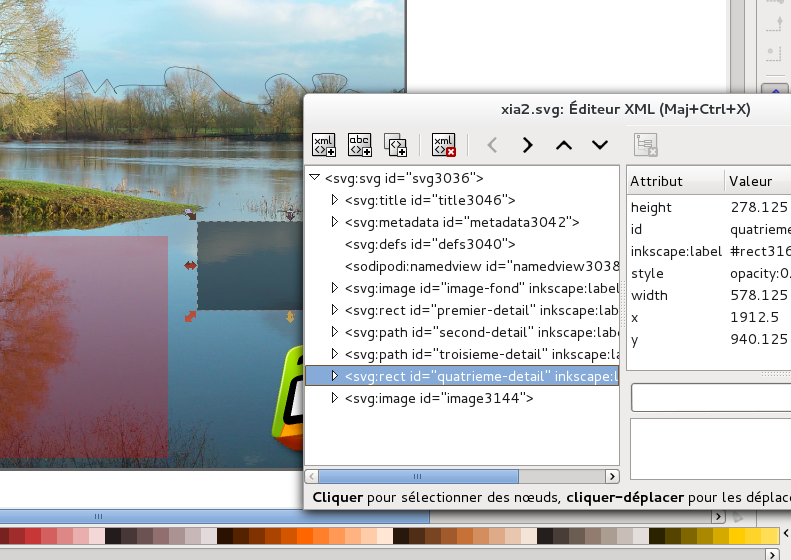
\includegraphics[width=\textwidth]{images/ordre_couches}
 \label{ordre_couches}
\end{figure}

\subsection{Abstract}

\begin{enumerate}
 \item One can enrich and shaping text using tags
 \item A multimedia enrichment is possible through a simple link relative
or absolute to a file whose format is recognized by Xia
 \item Adding images to the background image is possible by importing them
 \item It is possible to modify the default behavior of a detail by changing its color 
background (white, black)
 \item The order of the details in the image-active depends on the order
of their creation in Inkscape. Nevertheless, the Inkscape XML editor allows to change that order
\end{enumerate}


\section{Creating games with Xia}

Until now, this document has only talked about creation of traditionnal image-actives: 
background image enriched with cropped details associated with texts

This kind of image-active can be used in classrooms in various situations 
(students progressively discovering a document, or creating an image-active 
by themselves), but Xia introduces new features, 
such as the creation of games and activities, in which the final user 
has much more to do than simply clicking on details in order to read text.

\subsection{First game principle: selecting, finding elements in the image}

Explore the \href{http://geoffrey-gekiere.ac-versailles.fr/xia3}{image- 
active created for this section of the documentation} and download the \href
{http://geoffrey-gekiere.ac-versailles.fr/xia3/svg/xia3.svg}{svg} source file.
\textit{The game principle described in this section consists in selecting details 
on a background image. When the user has reached the goal described in the 
instructions, a message appears in a final pop up.}

This kind of game is almost the easiest way to create an image-active.
The designer only has to crop the details that the final user will have to select. 

The instructions have to be completed in the 
documents metadata. Xia will look into 
the informations  filled in the  \chemin
{Description} field of the metadata of the document (see section \ref{preparation_svg} and illustration \ref{titre_ia}), and create an instruction «~pop up~» 
that will show up at the opening of the game. The final user will just have to 
read the instructions and close the pop up to play the game.

When the user completes the game, a message automatically appears.  This message 
has to be filled in the \chemin{Description} field of the \chemin{Object Properties} of the 
background image \footnote{When creating a «~traditional~» image-active, 
this field creates the introduction text, not related with any detail 
(see section \ref{preparation_svg}).}.  Two informations are needed in order for this message to pop up 
: exact number of details that have to be selected and the message itself\footnote{This number does 
not have to match the number of details on the image) 
and the message itself.} This table sums up the tags that have to be used:

% le multicolumn refuse le \verb... à corriger
\begin{center}
 \begin{tabular}{|l|p{2in}|p{2in}|}
 % \hline
% \multicolumn{3}{|c|}{Informations à renseigner dans le champs Description des Propriétés de l'objet}\\
 \hline
  Goal & Enter the number of correct answers needed to complete the game & Display a message\\
  \hline
  Tag & \verb|<score></score>| & \verb|<message></message>|\\
  \hline
  Example & \multicolumn{2}{|l|}{<score>6</score>}\\
   & \multicolumn{2}{|l|}{<messageCongratulations!}\\
    & \multicolumn{2}{|l|}{You have completed the game!</message>}\\
  \hline
 \end{tabular}
\end{center}

\begin{wrapfigure}{r}{45mm}
  \centering
  
\includegraphics[scale=0.7]{./images/game1clic} 
\end{wrapfigure}

A little tip: text inserted inside the \verb|<message></message>| tag can be 
enriched. Images, videos or sounds can be inserted inside this message.
It is also possible to insert a link, allowing users to play another game.
in order to "chain" activities up by degree of difficulty.

The template \chemin{game1clic} should be chosen for any image-active matching 
the click to select game principle.



\subsubsection{Advanced image-active creation tips... How to show the user's progress in the use of a game game1clic ?}\label{détail_progression}

It is possible to automatically display graphical elements when users correctly 
select a correct answer.Those graphical elements being png imported images or 
shapes directly designed in Inkscape. But as Xia considers as a clickable 
detail any shapes designed using Inkscape tools, designer of the image-active 
will have to transform thoses shapes in bitmap, using the "bitmap copy" Inkscape tool. 
For example :
\begin{enumerate}
 \item Draw  a star of yellow sides on a yellow background with the  Inkscape tools 
d'Inkscape
 \item Select this star, and click on the \chemin{Edition} menu, then on \chemin{Make a bitmap copy}
 \item Delete the original star used to create the bitmap copy
\end{enumerate}

When the graphical elements are imported (png files) or created (bitmap copy 
of figures created by hand), just apply to those elements the following 
charasteristic :
\begin{center}
\chemin{Interactivity > OnClick} = \verb|off|
\end{center}
Then, group the clickable detail to its graphical element (by successively 
clicking on the detail and the graphical element with the Maj keystroke on),
then selecting \chemin{Group} in the Inkscape menu \chemin{Object}.

\subsubsection{Advanced image-active creation tips... How to highlight the user errors in a game1clic image-active?}

Games based on the details selection principle are obviously very
interesting educational games\ldots but it is also quite obvious to guess how some students may be tempted to cheat to achieve such games (for example, by 
frenetically clicking anywhere possible on the image, until the final message pops up).

This is why it may be interesting to be able to 
highlight the users errors during the game.

In order to do that, the image-active designer will anticipate users hypothetical mistakes, and 
put on the background image explicit graphical elements symbolizing those errors. 
This grapical element may be an imported image 
(png file) or a shape directly designed with the Inkscape tools, 
then converted into bitmap (see how to do that in the section 
\ref{détail_progression}). Those elements will have to possess the following characteristic:
\begin{center}
\chemin{Interactivity > OnClick} = \verb|disable-score| 
\end{center}
When applied with a \verb|disable-score| tag, a detail still remains clickable, but does not 
add a score to the counter that delivers the final success message pop up.

\subsection{Second game principle: classyfying, ordering, ranking}

\textit{The second kind of game that can be created with Xia consists in dragging and dropping graphical elements 
on the background image. If all the elements have been dropped on their corresponding drop zone, a pop up
message appears, confirming the achievement of the game}

Explore the \href{http://geoffrey-gekiere.ac-versailles.fr/xia5}{image-
active created for this section of the documentation} and download the \href
{http://geoffrey-gekiere.ac-versailles.fr/xia5/svg/xia5.svg}{svg} source file.

Here's how to create a game based on the drag and drop principle :
\begin{enumerate}
 \item In Inkscape:
\begin{itemize}
 \item Choose a background picture
 \item Create the graphical elements users of the image-active will have to drag and drop (ie. images or group of words)
 \item Using metadatas indicated, make each label matches its drop zone (actually being cropped details)
\end{itemize}
 \item In Xia
 \begin{itemize}
  \item Export the svg source file using the «~gameDragAndDrop~» template
 \end{itemize}
\end{enumerate}

Two methods can be used to create the drag and drop "graphical-elements".
A very simple way is to use a screenshot tool, in order to create png files, and then import them in Inkscape.
It is also possible to create those elements directly in Inkscape, by creating a text, grouping it with a shape,
and finally making a bitmap copy of this group 
(see section \ref{détail_progression})\footnote{\ldots do not forget to delete
the original text and shape group once the bitmap copy has been created.}.
The graphical elements then have to be associated with their drop zone \footnote{\textbf{One} object can match only \textbf{one} drop zone.}.

You will find in this table the metadatas to be filled in the \chemin
{Object Properties} of the drag and drop graphical elements and the corresponding details in order "to-twin" them :

\begin{center}
\begin{tabular}{|p{1.in}|p{2.5in}|p{1.5in}|}
\hline
 & Graphical element (drag and drop objects in the game) & Cropped detail (drop zone)\\
\hline
ID Field & & \verb|Detail_Title|\\
\hline
Description Field & \verb|<target>Detail_Title</target>| & \\
\hline
\end{tabular}
\end{center}

\begin{wrapfigure}{r}{45mm}
  \centering
  
\includegraphics[scale=0.7]{./images/gameDragAndDrop} 
\end{wrapfigure}


The designer let Xia know how the graphical elements match the drop zones by 
making the \chemin{ID} field of the drop zone 
with the \chemin{Description} field of the drag and drop graphical element. 
The only subtlety consists in the  \verb|<target></target>| tags that have to be filled in the \chemin
{Description} field.

Generating an image-active having the drag and
drop game principle corresponds in Xia in export \chemin{gameDragAndDrop}:



\subsubsection{How to add a «~magnet~» effect in the gameDragAndDrop template}

If the designer indicates\\
\begin{center}
\verb|<magnet>on</magnet>| 
\end{center}
in the \chemin{Description} field of the drop zone, a 
magnet effect will then be active when the final user will drop the graphical element on its matching drop zone.

The advantage of this option is that it allows the user to be sure 
that the non-resolution of the game comes from a mismatch of his 
labels, not a slight offset between the label and the drop zone.

\subsection{Abstract}

This table sums up the tags that have to be indicated when a game is created 
 (export game1clic or gameDragAndDrop) :

\begin{center}
 \begin{tabular}{|p{1.5in}|p{1in}|p{1in}|p{1in}|p{1in}|}
 \hline
 Tags & Role  & Element & Where ? & What ?\\
 \hline
 \verb|<score></score>| & Amount of correct answers needed to pop up the end message of the game & Background picture & Object properties $\rightarrow$ Description & Number corresponding to the required score\\
 \hline
 \verb|<message></message>| & Pops up the end message of the game & Background picture & Object properties $\rightarrow$ Description & A personalized message if necessary enriched with multimedia or html links\\
 \hline
 \verb|off| & Making a cropped detail unclickable & Detail & Object properties $\rightarrow$ Interactivty $\rightarrow$ Onclick & \\
 \hline
 \verb|disable-score| & Cropped detail is still clickable, but when clicked, does not add a point to the score game counter & Detail & Object properties $\rightarrow$ Interactivty $\rightarrow$ Onclick & \\
 \hline
 \verb|<target></target>| & Indicates the corresponding drag and drop element and drop zone & Graphical element to move & Object Properties $\rightarrow$ Description & Make sure to match the ID field of the drop zone\\
 \hline
 \verb|<magnet>on</magnet>| & Add a "magnet" effect & Drop zone & Object Properties $\rightarrow$ Description & \\
 \end{tabular}
\end{center}


\end{document}
